\documentclass[a4paper, 9pt]{report}
  
\author{Federico Mainetti Gambera}
\usepackage{amsmath}
\usepackage{amssymb}
\usepackage{graphicx}
\usepackage[italian]{babel}
\usepackage{import}
\usepackage{xifthen}
\usepackage{pdfpages}
\usepackage{transparent}
\usepackage{xcolor}
\usepackage{cancel}
\usepackage[a4paper,left=35mm,top=26mm,right=26mm,bottom=15mm]{geometry}
\usepackage{color}
\usepackage{tcolorbox}
\usepackage{hyperref}
\usepackage{makeidx}
\makeindex
\definecolor{lightgray}{gray}{0.75}
\renewcommand{\familydefault}{\sfdefault}
\newenvironment{rcases}
  {\left.\begin{aligned}}
  {\end{aligned}\right\rbrace}
\newcommand{\incfig}[1]{%
    \def\svgwidth{\columnwidth}
    \import{../images/}{#1.pdf_tex}
}
\begin{document}
\subsection*{TRIGONOMETRIA}
\[
    sin^2(x) + cos^2(x) = 1
\]
\[
    sin(2x) = 2sin (x)cos(x)
\]
\[
    sin(x) cos(x) = \frac{1}{2}sin(2x)
\]
\[
    cos(2x) = \begin{cases}
        cos^2(x) -sin^2(x)\\
        1-2sin^2(x)\\
        2cos^2(x)-1
    \end{cases}
\]
\[
    sin^2(x) = \frac{1}{2} (1-cos(2x)) \;\;\;\; ottenuta \; da \;[cos(2x) = cos^2(x) - sin^2(x) = 1 - 2 sin^2(x)]
\]
\[
    cos^2(x) = \frac{1}{2}(1+cos(2x)) \;\;\;\; ottenuta \; da \; [cos(2x) = cos^2(x) - sin^2(x) = 2cos^2(x) - 1]
\]
\[
    Ch^(x) = \frac{e^x + e^{-x}}{2}
\]
\[
    Sh^(x) = \frac{e^x - e^{-x}}{2}
\]
\[
    Ch^2(x) - Sh^2(x) = 1
\]
\[
    Sh(2x) = 2Sh(x)Ch(x)
\]
\[
    Ch(2x) = Sh^2(x) + Ch^2(x)
\]
\[
    SettSh(x) = log(+ + \sqrt{x^2+1})
\]
\[
    SettCh(x) = log(x + \sqrt{x-1} \cdot \sqrt{x+1})
\]
\[
    Sh(SettCh(a))= \sqrt{a^2-1} \;\;\;\; ottenuta \; da \; [Ch^2(x) -Sh^2(x) = 1] \rightarrow [Sh(x) = \sqrt{Ch^2(x) -1}] \rightarrow [x = SettCh(a)]
\]
\[
    Ch(SettSh(a))=\sqrt{a^2+1} \;\;\;\; ottenuta \; da \; [Ch^2(x) -Sh^2(x) = 1] \rightarrow [Ch(x) = \sqrt{1 + Sh^2(x)}] \rightarrow [x = SettSh(a)]
\]
\[
    sin(a)cos(b)=\frac{1}{2}sin(a+b)+sin(a-b)
\]
\[
    cos(a)sin(b)=\frac{1}{2}sin(a+b)-sin(a-b)
\]
\[
    cos(a)cos(b)=\frac{1}{2}cos(a+b)+cos(a-b)
\]
\[
    sin(a)sin(b)=-\frac{1}{2}cos(a+b)- cos(a-b)
\]
\[
    sin(a+b) =sin(a)cos(b) + sin(b) cos(a)
\]
\[
    sin(a-b) = sin(a)cos(b) - sin(b)cos(a)
\]
\[
    cos(a+b) = cos(a)cos(b) - sin(a)sin(b)
\]
\[
    cos(a-b)=cos(a)cos(b) + sin(a)sin(b)
\]
\[
    sin(\alpha) + sin(\beta) = 2 sin\left(\frac{\alpha + \beta}{2}\right) cos \left(\frac{\alpha - \beta}{2}\right)
\]
\[
    sin(\alpha) - sin(\beta) = 2 cos\left(\frac{\alpha + \beta}{2}\right) sin\left(\frac{\alpha - \beta}{2}\right)
\]
\[
    cos(\alpha) + cos(\beta) = 2 cos\left(\frac{\alpha + \beta}{2}\right) cos\left(\frac{\alpha - \beta}{2}\right)
\]
\[
    cos(\alpha) - cos(\beta) = -2sin\left(\frac{\alpha + \beta}{2}\right) sin\left(\frac{\alpha - \beta}{2}\right)
\]
\begin{figure}[h!]
    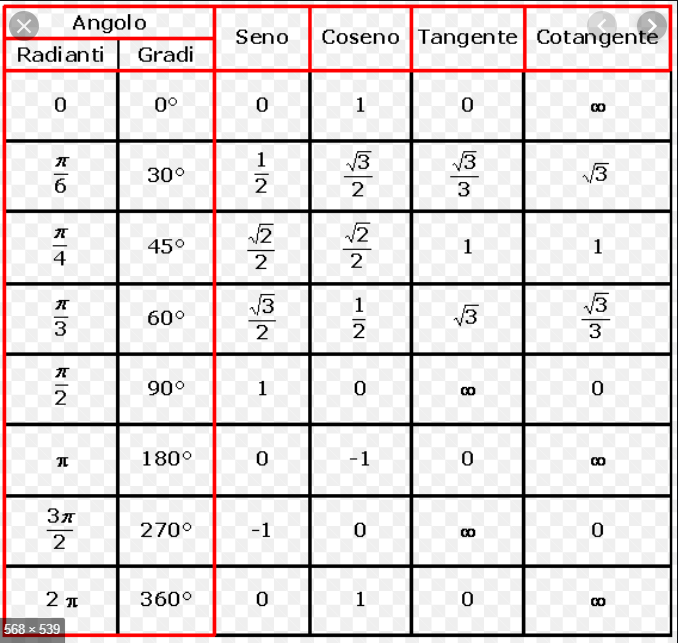
\includegraphics[width=300px]{../dim/trigonometria.PNG}
\end{figure}
\newpage
\subsection*{ASINTOTICI}
\begin{figure}[h!]
    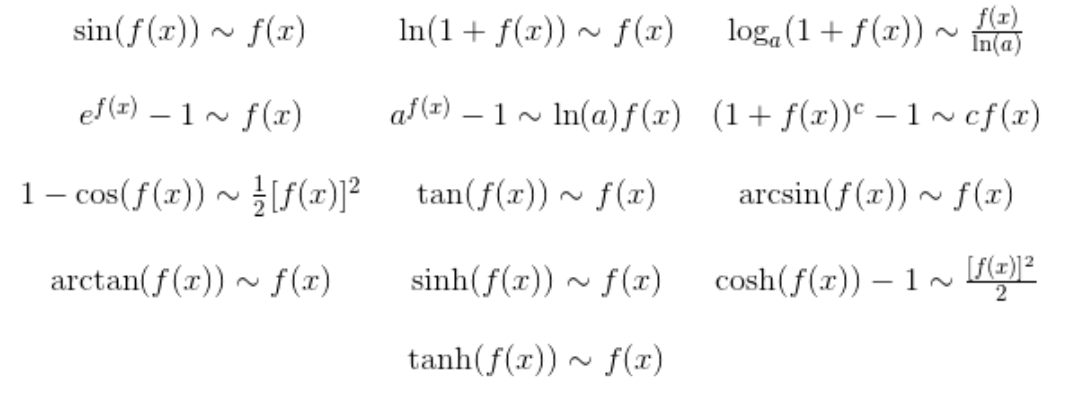
\includegraphics[width=\linewidth]{../dim/asintotici.PNG}
\end{figure}
\newpage
\subsection*{DERIVATE}
\begin{figure}[h!]
    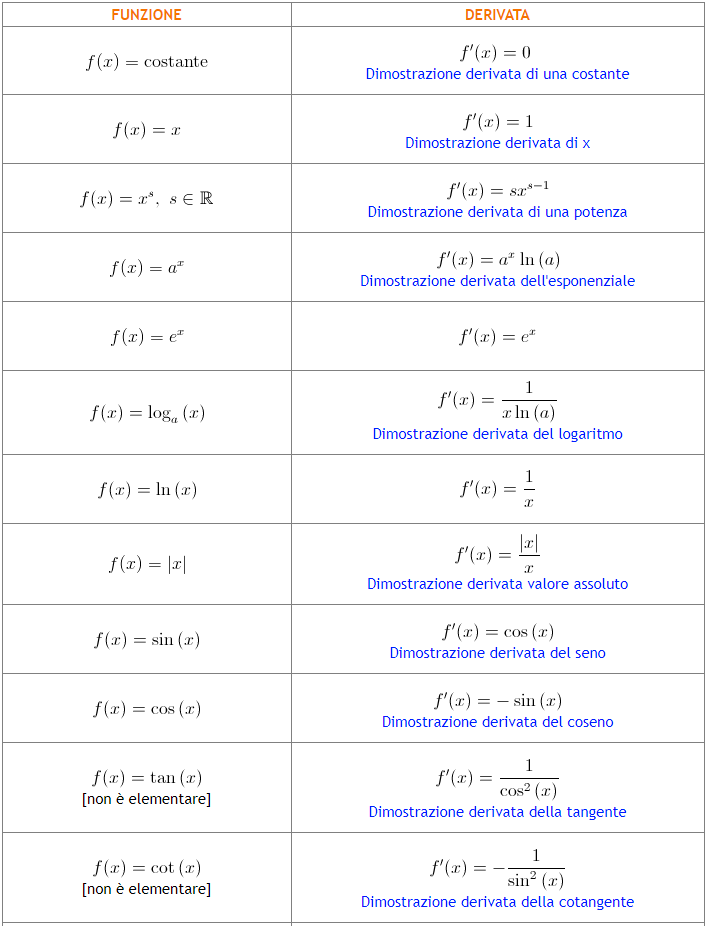
\includegraphics[width=\linewidth]{../dim/derivate1.PNG}
\end{figure}
\newpage
\begin{figure}[h!]
    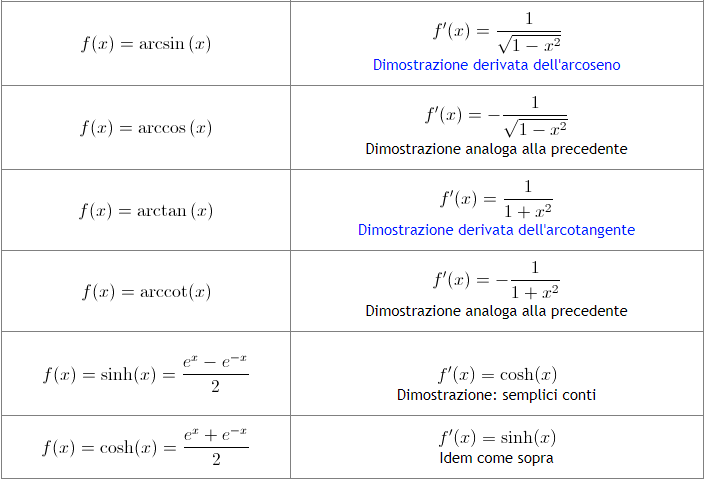
\includegraphics[width=\linewidth]{../dim/derivate2.PNG}
\end{figure}
\newpage
\subsection*{SVILUPPI}
\begin{figure}[h!]
    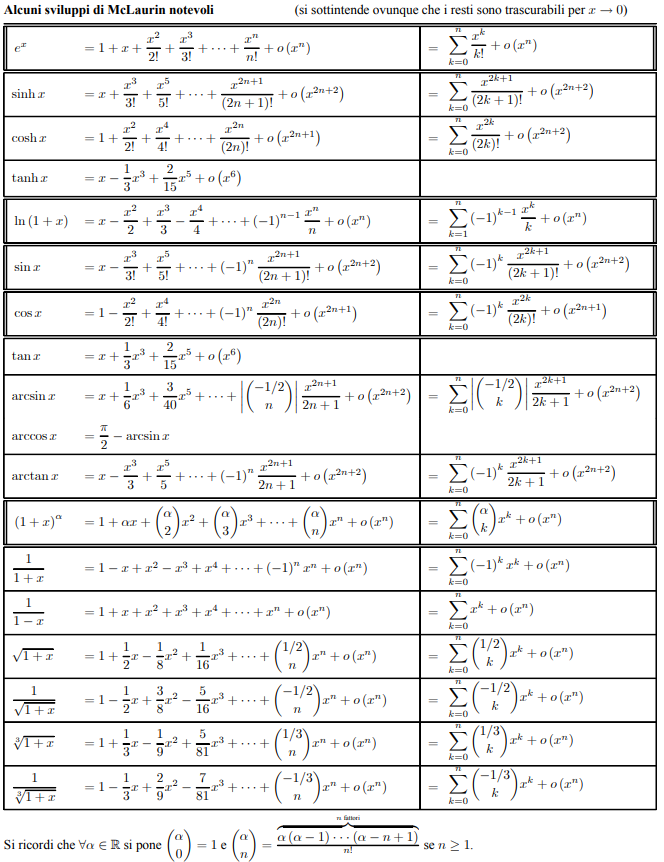
\includegraphics[width=\linewidth]{../dim/mclaurin.PNG}
\end{figure}
\subsection*{SERIE}
\subsection*{serie geometrica}
per $q \neq 1$
\[
    \sum_{n=0}^{\infty}q^n = \frac{1-q^{n+1}}{1-q}
\]
per $q = 1$
\[
    \sum_{n=0}^{\infty}q^n = \begin{cases}
        \frac{1}{1-q} & se \;\; -1<q<1\\
        +\infty &se \;\; q \geq 1\\
        irregolare \;\;& se \;\; q\leq-1 
    \end{cases}
\]
\subsection*{serie armonica}
\[
    \sum_{n=1}^{\infty}\frac{1}{n} \geq log(n+1) \rightarrow +\infty
\]
per $\alpha \leq 1$ 
\[
    \sum_{n=1}^{\infty} \frac{1}{n^\alpha} \geq \sum_{n=1}^{\infty}\frac{1}{n} \rightarrow +\infty
\]
per $\alpha > 1$ 
\[
    \sum_{n=1}^{\infty} \frac{1}{n^\alpha} = converge
\]
per $\alpha = 2$
\[
    \sum_{n=1}^{\infty}\frac{1}{n^2} = \frac{\pi^2}{6} (\sim  \sum_{n=1}^{\infty} \frac{1}{n(n+1)} = serie \;\; di \;\; mengoli)
\]
\subsection*{serie di mengoli}
\[
    \sum_{n=1}^{\infty}\frac{1}{n(n+1)} = \sum_{n=1}^{\infty} \frac{1}{n}-\frac{1}{n+1} = 1- \frac{1}{n+1} \rightarrow 1
\]
\subsection*{sviluppi di Taylor delle funzioni elementari}
\[
    e^x = \lim_{n\rightarrow +\infty}\sum_{k=0}^{n} \frac{x^k}{k!} = \sum_{k=0}^{+\infty} \frac{x^k}{k!}
\]
\[
    sin (x) =\sum_{k=0}^{\infty}(-1)^k \frac{x^{2k+1}}{(2k+1)!} =  \frac{e^{ix} - e^{-ix}}{2}
\]
\[
    cos (x) =\sum_{k=0}^{\infty}(-1)^k \frac{x^{2k}}{(2k)!} =\frac{e^{ix} + e^{-ix}}{2}
\]
\subsection*{Serie di potenza}
Con $a_k$ costanti reali (o complesse) e $x$ variabile reale (o complessa)
\[
    \sum_{k=0}^{\infty}a_k x^k
\]
\[
    Sh (x) = \sum_{k=0}^{\infty} \frac{x^{2k+1}}{(2k+1)!}
\]
\[
    Ch(x) = \sum_{k=0}^{\infty} \frac{x^{2k}}{(2k)!}
\]
\[
    log(1+x)= \sum_{k=1}^{\infty} (-1)^{k+1} \frac{x^k}{k} \;\;\; per \;\; |x|<1
\]
per $\alpha \in \mathbb{R}$
\[
    (1+x)^\alpha = \sum_{k=0}^{\infty} \binom{\alpha}{k}x^k \;\;\; per \;\; |x|<1
\]
\textbf{teor.} Condizione necessaria affinché una serie $\sum_{n=0}^{\infty} a_n$ converga è che il termine generale $a_n$ tenda a zero. (Cioè perchè la serie converga, il termine $a_n$ deve tendere a zero, ma non per forza se il termine $a_n$ tende a zero allora la serie converge)\newline
\newline
\textbf{teor.}supponiamo che una serie $\sum_{n=0}^{\infty} a_n$ converga, allora per ogni $k$ anche risulta convergente anche $\sum_{n=k}^{\infty} a_n$.\newline
\newline
\textbf{Criterio serie a termini non negativi} Una serie $\sum_{n=0}^{\infty}a_n$ a termini non negativi è convergente o divergente a $+\infty$. Essa converge se e solo se la successione delle somme parziali n-esime è limitata.\newline
\newline
\textbf{Criterio del confronto} Siano $\sum an$ e $\sum b_n$ due serie a termini non negativi tali che $a_n<b_n$ definitivamente, allora:
\begin{itemize}
    \item $\sum b_n$ convergente $\Rightarrow \sum a_n$ convergente. 
    \item $\sum a_n$ divergente $\Rightarrow \sum b_n$ divergente. 
\end{itemize}
\textbf{Criterio del confronto asintotico} Se $a_n \sim b_n$, allora le corrispondenti serie $\sum a_n$ e $\sum b_n$ hanno lo stesso carattere (o entrambe divergenti o entrambe divergenti )\newline
\newline
\textbf{Criterio della radice} Sia $\sum a_n$ una serie a termini non negativi. Se esiste il limite 
\[
    \lim_{n\rightarrow +\infty}\sqrt[n]{a_n} = l
\]
\begin{itemize}
    \item $l>1$ la serie diverge $+\infty$
    \item $l<1$ la serie converge
    \item $l=1$ nulla si può concludere
\end{itemize}
Spesso utilizzato con termini che hanno come esponente $n$.
\textbf{Criterio del rapporto} Sia $\sum a_n$ una serie a termini positivi. Se esiste il limite 
\[
    \lim_{n\rightarrow +\infty} \frac{a_{n+1}}{a_n} = l
\]
\begin{itemize}
    \item $l<1$ diverge $+\infty$
    \item $l<1$ converge 
    \item $l=1$ nulla si può concludere
\end{itemize}
Spesso utilizzato quando si hanno termini come $n^n$ e $n!$.
\textbf{Criterio serie a termini di segno variabile} Una serie $\sum a_n$ si dice assolutamente convergente se converge la serie $\sum |a_n|$. Se la serie $\sum a_n$ converge assolutamente, allora converge.\newline
\newline
\textbf{Criterio di Leibniz} Sia data la serie 
\[
    \sum_{n=0}^{\infty}(-1)^n a_n \;\; con  \;\; a_n\geq 0 \;\forall\;n
\]
Se la successione $\{a_n\}$ è decrescente e se $a_n \rightarrow 0$ per $n \rightarrow \infty$, allora la serie è convergente.\newline
Il criterio di Leibniz può essere applicato anche se i termini sono definitivamente di segno alterno e la successione $a_n$ è definitivamente decrescente.\newline
Per verificare la decrescenza bisogna dimostrare che $a_{n+1}<a_n$ oppure mediante il limite a $+ \infty$ della derivata prima di $a_n$ o studiano quando la derivata prima di $a_n<0$ .\newline
\newline
\textbf{Criterio della somma di serie convergenti} Se $\sum_{n=1}^{\infty} a_n$ converge e $\sum_{n=1}^{\infty} b_n$ converge, allora $\sum_{n=1}^{\infty} a_n +b_n$ converge.\newline
\newline
\textbf{Criterio della somma di serie convergenti e divergenti} Se $\sum_{n=1}^{\infty} a_n$ converge e $\sum_{n=1}^{\infty} b_n$ diverge, allora $\sum_{n=1}^{\infty} a_n + b_n$ diverge.\newline
\newline
\textbf{Criterio serie a termini complessi} Sia la serie $\sum_{n=0}^{\infty} a_n$ con $a_n$ complesso, se la serie  $\sum_{n=0}^{\infty} |a_n|$ converge, allora anche $\sum_{n=0}^{\infty} a_n$ converge \newline
\newline
\textbf{Criterio di Dirichlet} Siano $a_n$ e $b_n$ due succesioni tali che:
\begin{itemize}
    \item $a_n$ è a valori complessi e la sua successione delle somme parziali è limitata.
    \item $b_n$ è a valori reali positivi e tende monotonamente a zero
\end{itemize}
allora la serie $\sum a_nb_n$ è convergente.



\subsection*{INTEGRALI}
\subsection*{Teorema fondamentale del calcolo integrale:}
\[
    \int_{a}^{b} f(x) dx = G(b) - G(a)
\]
\subsection*{Proprietà degli integrali:}
\[
    \int_{a}^{b} f(x)dx = \int_{a}^{r} f(x) dx + \int_{r}^{b} f(x) dx
\]
\[
    \left| \int_{a}^{b} f(x) dx \right| \leq \int_{a}^{b} |f(x)| dx
\]
\[
    \int k \cdot f(x) dx = k \cdot \int f(x) dx
\]
\[
    \int [f_1(x) + f_2(x) ] dx= \int f_1(x) dx + \int f_2(x) dx
\]
\subsection*{Integrali fondamentali:}
\[
    \int f'(x) dx = f(x) +c
\]
\[
    \int a \; dx = ax +c
\]
\[
    \int x^n dx = \frac{x^{n+1}}{n+1} +c
\]
\[
    \int \frac{1}{x}dx = ln(|x|) +c
\]
\[
    \int sin(x) dx = -cos(x) +c
\]
\[
    \int cos(x) dx = sin(x)+c
\]
\[
    \int tan(x) dx = -log|cos(x)| +c
\]
\[
    \int log(x) dx \;\; = xlog(x) - \int x \cdot  \frac{1}{x} dx - \int 1 dx = x log(x) -x + c
\]
\[
    \int arctg (x) dx \;\; = x arctg(x) -\int \frac{x}{1+x^2}dx = x arctg(x) -\frac{1}{2}log(1+x^2) + c 
\]
\[
    \int cotg(x) dx = log|sin(x)| +c
\]
\[
    \int (1+tg^2(x))dx = \int \frac{1}{cos^2(x)} dx = tg(x) +c
\]
\[
    \int (1+ctg^2(x))dx = \int \frac{1}{sin^2(x)} dx = -cotg(x) +c
\]
\[
    \int Sh(x) dx = Ch(x) +c
\]
\[
    \int Ch(x) dx = Sh(x) +c
\]
\[
    \int Th(x) dx = log(Ch(x))+c
\]
\[
    \int Coth(x) dx = log|Sh(x)| +c
\]
\[
    \int e^x dx = e^x+c
\]
\[
    \int e^{kx} dx = \frac{e^{kx}}{k} +c
\]
\[
    \int a^x dx = \frac{a^x}{ln(a)}+c
\]
\subsection*{Integrali notevoli:}
\[
    \int sin^2(x) dx = [integrato \; una \; volta \; per \; parti \; e \; sostituzione \; con \; cos^2(x)+ sin^2(x) = 1] = \frac{1}{2}(x-sin(x)cos(x)) +c
\]
\[
    \int cos^2(x) dx = [integrato \; una \; volta \; per \; parti \; e \; sostituzione \; con \; cos^2(x)+ sin^2(x) = 1] = \frac{1}{2}(x+sin(x)cos(x)) +c
\]
\[
    \int tan^2(x) dx = tan(x) -x +c
\]
\[
    \int cotan^2(x) dx = -x -cot(x) +c 
\]
\[
    \int Sh^2(x) dx = [integrato \; una \; volta \; per \; parti \; e \; sostituzione \; con \; Ch^2(x) - Sh^2(x) = 1] = \frac{1}{4}(Sh(2x)-2x) +c
\]
\[
    \int Ch^2(x) dx = [integrato \; una \; volta \; per \; parti \; e \; sostituzione \; con \; Ch^2(x) - Sh^2(x) = 1] = \frac{1}{2}(x + Sh(x)Ch(x)) +c
\]
\[
    \int Th^2(x) dx = x - Th(x) +c 
\]
\[
    \int Coth^2(x) dx = x - Coth(x) +c 
\]
\[
    \int \frac{1}{sin^2(x)} dx = [1 = cos^2(x) +sin^2(x)] = \int 1 + tan^2(x) dx = -cotan(x) + c
\]
\[
    \int \frac{1}{cos^2(x)} dx = [1 = cos^2(x) +sin^2(x)] = \int 1 + cotan^2(x) dx = tan(x) + c
\]
\[
    \int \frac{1}{tan^2 (x)} dx = \int cotan^2(x) dx 
\]
\[
    \int \frac{1}{cotan^2(x) }dx = \int tan^2(x) dx 
\]
\[
    \int \frac{1}{Ch^2(x)} dx = \int (1-Th^2(x))dx= Th(x)+c
\]
\[
    \int \frac{1}{Sh^2(x)} = \int (-1 Coth^2(x)) dx = -Coth(x) +c
\]
\[
    \int \frac{1}{1+x^2} dx = arctg(x) +c
\]
\[
    \int \frac{1}{1-x^2} dx = \frac{1}{2}log\left|\frac{1+x}{1-x}\right|+c
\]
\[
    \int \frac{1}{\sqrt{1+x^2}} dx = arcSh(x) +c = log(x + \sqrt{1+x^2}) +c
\]
\[
    \int \frac{1}{\sqrt{1-x^2}} dx = arcsin(x) +c
\]
\[
    \int \frac{1}{\sqrt{-1 + x^2}} dx = log|x+ \sqrt{x^2-1}| +c
\]
\[
    \int \frac{1}{\sqrt{\pm a^2 + x^2}} dx = log|x + \sqrt{x^2 \pm a^2}|+c
\]
\[
    \int \sqrt{x^2 \pm a^2} dx = \frac{x}{2} \sqrt{x^2 \pm a^2} \pm \frac{a^2}{2} log(x + \sqrt{x^2 \pm a^2}) +c
\]
\[
    \int \sqrt{a^2 - x^2}dx = \frac{1}{2}(a^2arcsin(\frac{x}{a}) + x \sqrt{a^2 - x^2} )+c
\]
\subsection*{Integrali riconducibili:}
\[
    \int f^n(x) \cdot f'(x) dx = \frac{f^{n+1}(x)}{n+1} +c
\]
\[
    \int \frac{f'(x)}{f(x)} dx = log|f(x)|+c
\]
\[
    \int f'(x) \cdot cos(f(x)) dx =  sin(f(x))+c
\]
\[
    \int f'(x) \cdot sin(f(x)) dx = -cos(f(x)) +c
\]
\[
    \int e^{(f(x)} \cdot f'(x) dx = e^{f(x)}+c
\]
\[
    \int a^{f(x)} \cdot f'(x) dx = \frac{a^{f(x)}}{ln(a)} +c
\]
\[
    \int \frac{f'(x)}{1+f^2(x)} dx = arctg(f(x))+c
\]
\subsection*{Integrazione per sostituzione:}
Sostituire alla variabile $x$ una funzione di un'altra variabile $t$, purchè tale funzione sia derivabile e invertibile.\newline
Ponendo $x = g(t)$ da cui deriva $dx = g'(t) dt$ si ha che:
\[
    \int f(x) dx = \int f[g(t)] \cdot g'(t) dt
\]
Da ricordare è che se si è in presenza di un integrale definito bisogna aggiornare anche gli estremi di integrazione. Se non si volesse cambiare l'intervall odi integrazione si può risostituire il vecchio valore di $t$.
\subsection*{Integrazione delle funzioni razionali:}
\[
    \int \frac{P_n(x)}{Q_m(x)} dx
\]
Per prima cosa se il grado del numeratore è $\geq$ del grado del denominatore, si esegue la divisione di polinomi:
\begin{itemize}
    \item Si dispongono i polinomi dal termine di grado maggiore a quello minore nella seguente maniera:
    \[
        P(x) \;\; | \;\; Q(x)    
    \]
    badando al fatto che se nel polinomio $P(x)$ mancasse qualche termine bisognerebbe scrivere $0$ nella sua posizione.
    \item Si dividono il termine di grado massimo di $P(x)$ con quello di grado massimo di $Q(x)$, riportando il risultato al di sotto di $Q(x)$.
    \item Moltiplichiamo il termine appena scritto per ogni termine di $Q(x)$, ne invertiamo il segno e lo trascriviamo al di sotto dei termini con lo stesso grado di $P(x)$
    \item Sommiamo termine per termine $P(x)$ con i valore appena scritti e li riportiamo sotto.
    \item Ripetiamo questo procedimento finchè il grado più alto fra i termini dell'ultima riga scritta a sinistra è minore (non minore uguale) del termine di grado massimo di $Q(x)$
    \item Il polinomio a destra è il risultato della divisione $S(x)$, mentre ciò che rimane sulla sinistra è il resto $R(x)$. Possiamo ora riscrivere il numeratore:
    \[
        P(x) = S(x) \cdot Q(x) + R(x)
    \]
\end{itemize}
Vediamo ora i vari casi possibili:
\begin{itemize}
    \item \textbf{denominatore di primo grado:} integrale immediato tramite il logaritmo
    \item \textbf{denominatore di secondo grado:} si calcola il segno del discriminante:
    \begin{itemize}
        \item \textbf{due radici distinte:} si scompone in fratti semplici
        \[
            \frac{N(x)}{D_1(x) \cdot D_2(x)} = \frac{a}{D_1(x)} + \frac{b}{D_2(x)}
        \]
        \[
            \frac{a \cdot D_2(x) + b \cdot D_1(x)}{D_1(x) \cdot  D_2(x)} = \frac{N(x)}{D_1(x) \cdot D_2(x)}
        \]
        \[
            a \cdot D_2(x) + b \cdot D_1(x)= N(x)
        \]
        Una volta determinate $a$ e $b$ si riscrive l'integrale come $\frac{a}{D_1(x)} + \frac{b}{D_2(x)}$ e si integra come somma di logaritmi
        \item \textbf{denominatore quadrato perfetto:} (due soluzioni coincidenti), si procede per sostituzione:
        \[
            \int \frac{N(x)}{D(x)^2} dx = [D(x) = t, \; \dots] = \; \dots
        \] 
        L'utilità della sostituzione è quella di spezzare la frazione in una somma di frazion ida integrare una ad una.
        \item \textbf{denominatore non si annulla mai:}\newline
        Casi semplici:
        \[
            \int \frac{1}{1 + x^2}dx = arctg (x) +c
        \]
        \[
            \int \frac{1}{x^2 + a^2}dx = \frac{1}{a} arctg \frac{x}{a} +c
        \]
        \[
            \int \frac{1}{a^2 + (x+b)^2}dx = \frac{1}{a} arctg \frac{x+b}{a} +c
        \]
        Caso generico: Si cerca di dividere l'integrale in una somma di integrali, il primo deve contenere al numeratore la derivata del denominatore, il secondo non deve contenere la $x$ al numeratore, cioè deve essere una costante e quindi riconducibile ai casi semplici sopra riportati. Il denominatore non cambia. Ci si arriva a logica. 
    \end{itemize}
    \item \textbf{denominatore di grado maggiore di due:} è sempre possibile scomporlo in prodotti di fattori di primo grado o di secondo grado irriducibili, per farlo si usa Ruffini (o altrimenti si va a tentoni ricordando che PROBABILMENTE una radice della funzione è un dividendo (positivi e negativi) del numero che si ricava moltiplicando il coefficiente del termine massimo e il termine noto).\newline
    Fatto questo si scompone la frazione in fratti semplici con la stessa logica del caso di due radici distinte, ricordando che il numeratore deve essere un espressione di un grado minore del denominatore, per esempio se il denominatore è di grado $2$, allora si userà $ax+b$ che è di grado $1$.
\end{itemize}
\subsection*{Funzioni razionali di $e^x$}
Si pone $e^x = t$, $x= log(t)$, $dx = \frac{dt}{t}$ e ci si riconduce a una funzione razionale classica.
\subsection*{Integrazione per parti:}
\[
    \int f'(x) \cdot  g(x) dx = f(x) \cdot g(x) - \int f(x) \cdot g'(x)dx
\]
La formula deriva dalla formula di derivazione della moltiplicazioni di due funzioni:
\[
    (fg)' = f'g + fg'
\]
\[
    fg' = (fg)' - f'g
\]
Si può vedere la formula di integrazione per parti più facilmente così:
\[
    \int integranda \cdot derivanda \; dx = primitiva \cdot derivanda - \int primitiva \cdot derivata \; dx
\]
L'integrazione per parti si usa:
\begin{itemize}
    \item dovendo calcolare integrali della forma
    \[
        \int x^n \cdot f(x) dx \;\;\; f(x) = \begin{cases}
            cos(x)\\ 
            sin(x)\\ 
            e^x\\ 
            Sh(x)\\ 
            Ch(x)        
        \end{cases}
    \]
    si integra per parti derivando $x^n$ e integrando $f(x)$. Per $n=1$ l'integrale si riduce a uno immediato, per $n>1$ si itera il procedimento fino al caso $n=1$. Si possono svolgere allo stesso modo anche integrali del tipo:
    \[
        \int P_n(x) f(x) dx
    \]
    \item dovendo calcolare integrali della forma
    \[
        \int f(x) g(x) dx \;\;\;\; \begin{cases}
            f(x) = e^{\alpha x}, Sh(\alpha x), Ch( \alpha x), a^{bx} \\
            g(x) = cos( \beta x), sin(\beta x)
        \end{cases}
    \]
    si eseguono due integrazioni per parti consecutive, nella prima la scelta della funzione da integrare o derivare è indifferente, nella seconda però la scelte deve essere coerente alla prima. Chiamando $I$ l'integrale di partenza si ottiene una funzione della forma
    \[
        I = h(x) - \frac{\beta}{\alpha}^2 I
    \]
    da cui si ricava $I$.\newline
    Se entrambe le funzioni $f(x)$ e $g(x)$ sono del tipo $cos(x)$ o $sin(x)$ si usano le formule di duplicazione o prostaferesi (vedi più avanti).
    \item L'integrale del logaritmo, derivando $log(x)$ e integrando $1$
    \[
        \int log(x) dx \;\; = xlog(x) - \int x \cdot  \frac{1}{x} dx - \int 1 dx = x log(x) -x + c
    \]
    Più in generale, dovendo calcolare integrali della forma
    \[
        \int x^m log^n(x) dx
    \]
    e ponendo $g' = x^m$ e $f = log^n(x)$ ed eseguendo iterativamente $n$ integrazioni per parti si riesce a calcolare l'integrale del logaritmo. Ancora più in generale si possono risolvere integrali della forma:
    \[
        \int P_m(x) \cdot Q_n(log(x)) dx 
    \]
    \item l'integrale dell'arcotangente, derivando $arctg(x)$ e integrando $1$
    \[
        \int arctg (x) dx \;\; = x arctg(x) -\int \frac{x}{1+x^2}dx = x arctg(x) -\frac{1}{2}log(1+x^2) + c 
    \]
    Più in generale
    \[
        \int x^n arctg(x) dx  = \frac{x^{n+1}}{n+1}arctg(x) - \int\frac{x^{n+1}}{n+1} \frac{dx}{1+x^2}
    \]
\end{itemize}
\subsection*{integrazione delle funzioni trigonometriche}
\begin{itemize}
    \item dovendo calcolare
    \[
        \int f(sin(x)) \cdot  cos(x) dx \;\;\; \Rightarrow  \;\;\; sin(x) = t, cos(x) dx =dt
    \]
    \[
        \int f(cos(x)) \cdot  sin(x) dx\;\;\; \Rightarrow  \;\;\; cos(x) ) t, -sin(x) dx = dt
    \]
    In particolare per calcolare 
    \[
        \int sin^n(x) cos^m(x)
    \]
    se almeno uno degli esponenti è dispari si riesce a riscrivere l'integrale in una delle forme viste sopra utilizzando: $sin^2(x) + cos^2(x) = 1$. Se entrambi gli esponenti sono pari si usano le formule trigonometriche per abbassarne il grado: $cos^2(x) = \frac{1}{2}(1+cos(2x))$ e $sin^2(x) = \frac{1}{2} (1-cos(2x))$
    \item per integrali del tipo
    \[
        \int cos(\alpha x) sin(\beta x) dx, \;\;\;\int cos(\alpha x) cos(\beta x) dx, \;\;\;\int sin(\alpha x) sin(\beta x) dx,
    \]
    si usano le regole di prostaferesi che riconducono a somme di integrali immediati
    \item integrali di funzioni razionali di $sin(x)$ e $cos(x)$ possono sempre essere ricondotti a integrali di funzioni razionali generiche tramite la sostituzione:
    \[
        t = tg\left(\frac{x}{2}\right), \;\;\; x= 2 arctg(t), \;\;\;dx = \frac{2}{1+t^2}dt
    \]
    ne derivano le seguenti identità trigonometriche:
    \[
        \begin{cases}
            cos(x) = \frac{1-t^2}{1+t^2}\\
            sin(x) = \frac{2t}{1+t^2}
        \end{cases}
    \]
    \item integrali definiti notevoli:
    \[
        \int_{0}^{n \frac{\pi}{2}}cos^2(kx) dx = \int_{0}^{n \frac{\pi}{2}}sin^2(kx) dx = n \frac{\pi}{4}
    \]
    \item per calcolare integrali razionali con $Sh(x)$ e $Ch(x)$ o si trovano scorciatoie con trasformazioni oppure si usa la sostituzione $e^x = t, x= log(t), dx = \frac{dt}{t}$
\end{itemize}
\subsection*{Integrazione delle funzioni irrazzionali}
\begin{itemize}
    \item se l'integranda è una funzione razionale di $x$ moltiplicata per solo una delle seguenti
    \[
        \int R(x) \sqrt{a^2-x^2} dx = [x=a \cdot  sin(t), dx =a \cdot  cos(t)dt] = \int \sqrt{a^2(1-sin^2(t))}dx = \int|a \cdot  cos(t)|dx
    \]
    \[
        \int R(x) \sqrt{a^2 + x^2} = [x=a \cdot  Sh(t), dx =a \cdot  Ch(t)dt] = \int \sqrt{a^2(1-Sh^2(t))}dx = \int a \cdot  Ch(t)dx
    \]
    \[
        \int R(x) \sqrt{x^2 -a^2} = [x=a \cdot  Ch(t), dx =a \cdot Sh(t)dt] = \int \sqrt{a^2(Ch^2(t)-1)}dx = \int|a \cdot Sh(t)|dx
    \]
    Negli ultimi due casi per tornare alla variabile x occorre usare le funzioni iperobliche inverse:
    \[
        \begin{cases}
            x = a \cdot  Ch(t) \Rightarrow t = SettCh(\frac{x}{a}) = log\left(\frac{x}{a}+\sqrt{\frac{x^2}{a^2}-1}\right)\\
            x= a \cdot Sh(t) \Rightarrow t = SettSh\left(\frac{x}{a}\right) = log\left(\frac{x}{a}+\sqrt{\frac{x^2}{a^2}+1}\right)
        \end{cases}
    \]
    è utile anche ricordare che $Sh(SettCh(a))= \sqrt{a^2-1}$ e $Ch(SettSh(a))=\sqrt{a^2+1}$
    \item integrale di una funzione razionale di $x, x^{\frac{n_1}{m_1}}, x^{\frac{n_2}{m_2}}$, etc. \newline
    Si pone $x = t^n$ con $n=$ minimo comune multiplo di $m_1$, $m_2$, etc. Si ha quindi $dx = n \cdot  t^{n-1} dt$ e si ottiene una funzione razionale di $t$.
    \item Se l'integranda è una funzione del tipo $R(x^{2n+1}, \sqrt{x^2 \pm a^2})$
    \[
        \int x^{2n+1}R(\sqrt{x^2 \pm a^2})dx = [\sqrt{x^2 \pm a^2} = t, xdx= tdt, x^{2n+1} \cdot dx = (t^2 \mp a^2)^n t \cdot  dt]
    \]
\end{itemize}
\subsection*{Simmetrie e valori assoluti nel calcolo di integrali definiti}
\begin{itemize}
    \item se $f(x)$ è \textbf{pari}:
    \[
        \int_{-k}^{k}f(x)dx = 2 \int_{0}^{k} f(x) dx
    \]
    \item se $f(x)$ è \textbf{dispari}:
    \[
        \int_{-k}^{k}f(x)dx = 0
    \]
\end{itemize}
\subsection*{Osservazione. Integrale generalizzato di una funzioen dispari su un intervallo simmetrico}
Non è corretto affermare l'annullarsi di un integrale dispari per motivi di simmetria in un intervallo simmetrico senza prima verificare la convergenza dell'integrale stesso.
\subsection*{INTEGRALI GENERALIZZATI}
\subsection*{Integrazione di funzioni non limitate}
Metodo generale di risoluzione:
\[
    \lim_{x\rightarrow b^-} f(x) = \pm \infty \;\;\;\;\;\;\;\;\;\;\;\;\;\;\;\;\;\;\;\;\;\;\;\;\;\;\;\;\;\;\;\;\;\;\;\;\;\;\;\;\lim_{x\rightarrow a^+}f(x) = \pm \infty
\]
\[
    \int_{a}^{b}f(x)dx = \lim_{\epsilon\rightarrow 0^+}\int_{a}^{b-\epsilon}f(x)dx \;\;\;\;\;\;\;\;\;\;\;\;\; \int_{a}^{b}f(x)dx = \lim_{\epsilon\rightarrow 0^+}\int_{a+\epsilon}^{b}f(x)dx 
\]
\subsection*{Criteri di integrabilità al finito}
Siano $\lim_{x\rightarrow b^-}f(x) = \lim_{x\rightarrow b^-}g(x) = + \infty$:
\begin{itemize}
    \item confronto: se $0\leq f(x) \leq g(x)$, allora $g$ integrabile $\Rightarrow f$ integrabile e $f$ non integrabile $\Rightarrow g$ non integrabile.
    \item confronto asintotico: se $f>0$ e $g>0$ e $f \sim g$ per $x \rightarrow b^-$, allora $f$ integrabile $\Leftrightarrow g$ integrabile.
    \item \textbf{teor.} (da usare per studiare per esempio funzioni seno e coseno per $x \rightarrow \infty$)
    \[
        \int_{a}^{b}|f(x)|dx \;\; convergente \;\;\Rightarrow \int_{a}^{b}f(x)dx \;\;convergente
    \]
\end{itemize}
\subsection*{Integrazione su intervalli illimitati}
Metodo generale di risoluzione:
\[
    \int_{a}^{+\infty}f(x) dx = \lim_{\omega\rightarrow +\infty}\int_{a}^{\omega}f(x)dx
\]
\[
    \int_{- \infty}^{b}f(x) dx = \lim_{\omega\rightarrow -\infty}\int_{\omega}^{b}f(x)dx
\]
\[
    \int_{-\infty}^{+\infty}f(x) dx = \int_{-\infty}^{c} f(x) dx + \int_{c}^{+\infty}f(x) dx
\]
\textbf{def.} Se il limite dell'integrale di $f$ esiste finito allora $f$ si dice integrabile oppure che l'integrale è convergente. \newline
\textbf{def.} Se il limite dell'integrale è $\pm \infty$, l'integrale si dice divergente.\newline
\textbf{def.} Se il limite non esiste, l'integrale non esiste.\newline
\textbf{per essere integrabile deve avere limite finito.}
\subsection*{Criteri di integrabilità all'infinito}
\begin{itemize}
    \item confronto: se $0\leq f(x) \leq g(x)$ in $[a,+\infty)$, allora $g$ integrabile $\Rightarrow f$ integrabile e $f$ non integrabile $\Rightarrow g$ non integrabile.
    \item confronto asintotico: se $f>0$, $g>0$ e $f \sim g$ per $x \rightarrow + \infty$, allora $f$ integrabile $\Leftrightarrow g$ integrabile
    \item \textbf{teor.} (da usare per studiare per esempio funzioni seno e coseno per $x \rightarrow \infty$)
    \[
        \int_{a}^{+\infty}|f(x)| dx \;\; convergente \;\; \Rightarrow \int_{a}^{+\infty} f(x) dx \;\;convergente
    \]
\end{itemize}
\subsection*{Osservazione. Ordine di annullamento di una funzione derivabile.}
Se $f$ è una funzione derivabile in un intervallo $I$, la formula di Taylor ci dice che se $f$ si annulla in un punto $\alpha \in I$, si annulla almeno del prim'ordine. Precisamente poichè
\[
    f(x) - f(\alpha) = f'(\alpha)(x-\alpha) + o(x-\alpha)
\]
se $f'(\alpha) \neq 0$ allora $f$ ha uno zero del prim'ordine in $\alpha$. Se $f'(\alpha) = 0$ ma, ad esempio, $f''(\alpha) \neq 0$, si può concludere che $f$ si annulla del $2^0$ ordine, e così via. In ogni caso non può annullarsi di un ordine inore di $1$.
\subsection*{Integrali generalizzati notevoli}
Caso 1:
\[
    \int_{a}^{b}\frac{1}{(x-a)^p}dx \rightarrow \begin{cases}
        converge \;\;&se \;\;p<1\\
        diverge \;\;&se \;\; p\geq 1
    \end{cases}
\]
\[
    \int_{a}^{b}\frac{dx}{(b-x)^p} \rightarrow  \begin{cases}
        converge \;\;&se \;\;p<1\\
        diverge \;\;&se \;\; p\geq 1
    \end{cases}
\]
Caso 2:
\[
    \int_{a}^{+\infty}\frac{1}{x^p}dx \rightarrow \begin{cases}
        converge \;\; & se \;\; p > 1\\
        diverge \;\; &  se \;\; p \leq 1
    \end{cases}
\]
Caso 3: con $0< \alpha < 1$
\[
    \int_{0}^{\alpha} \frac{1}{x^a \cdot  |ln(x)|^b} \rightarrow \begin{cases}
        converge \;\; se \;\; & \begin{cases}
            a < 1 \;\; e \;\; b \in \mathbb{R}\\
            oppure \\
            a=1 \;\; e \;\; b > 1
        \end{cases}\\
        diverge \;\; se \;\; & \begin{cases}
            a>1 \;\; e \;\; b \in \mathbb{R}\\
            oppure\\
            a=1 \;\; e \;\; b \leq 1
        \end{cases}
    \end{cases}
\]
Caso 4: con $\alpha > 1$
\[
    \int_{\alpha}^{+\infty} \frac{1}{x^\alpha \cdot ln^b(x)}dx \rightarrow \begin{cases}
        converge \;\; se \;\; & \begin{cases}
            a > 1 \;\; e \;\; b \in \mathbb{R}\\
            oppure \\
            a=1 \;\; e \;\; b > 1
        \end{cases}\\
        diverge \;\; se \;\; & \begin{cases}
            a<1 \;\; e \;\; b \in \mathbb{R}\\
            oppure\\
            a=1 \;\; e \;\; b \leq 1
        \end{cases}
    \end{cases}
\]
Caso 5: con $\alpha> 1$
\[
    \int_{1}^{\alpha}\frac{1}{ln^p(x)} dx \rightarrow \begin{cases}
        converge \;\; se \;\; &p<1\\
        diverge \;\; se \;\; &p\geq 1
    \end{cases}
\]
\subsection*{FUNZIONI INTEGRALI}
\textbf{teor.} Secondo teorema fondamentale del calcolo integrale \newline
Sia $f: [a,b] \rightarrow \mathbb{R}$ una funzione integrabile e sia $x_0 \in [a,b]$ e sia 
\[
    F(x) = \int_{x_0}^{x} f(t) dt
\]
Allora:
\begin{itemize}
    \item La funzione $F$ è continua in $[a,b]$
    \item Se inoltre $f$ è continua in $[a,b]$, allora $F$ è derivabile in $[a,b]$ e vale
    \[
        F'(x) = f(x) \;\; per \; ogni \; x \in[a,b]
    \]
    (Se $f(t)$ non è continua su tutto $I$, ma è integrabile in senso generalizzato, in tutti i punti in cui $f(t)$ è continua, $F(x)$ è derivabile e $F'(x) = f(x)$)\newline
    $F$ ha punti di non derivabilità dove $f$ è discontinua.
\end{itemize}
Conseguenze:
\begin{itemize}
    \item se $f$ è continua, $F$ è derivabile con continuità
    \item se $f$ è continua e derivabile con continuità, anche $F'$ è derivabile con continuità, quindi $F$ è due volte derivabile con continuità. Iterando: la funzione integrale ha sempre un grado di regolarità in più rispetto alla funzione integranda
    \item ogni fuzione continua su $I$ ha una primitiva su $I$
\end{itemize}
Logica degli esercizi in cui bisogna trovare l'intervallo di definizione:
\[
    F(x) = \int_{x_0}^{x}f(x)dx
\]
\begin{itemize}
    \item lo scopo è determinare dove la funzione integranda è integrabile.
    \item Vedere dove la funzione integranda è continua, una funzione continua è integrabile. Analizzare i punti di discontinuità:
    \item Se una funzione ha un numero finito di discontinuità limitate in un intervallo, allora è integrabile in quell'intervallo. In poche parole se è una discontinuità a salto è integrabile.
    \item Per gli altri punti di discontinuità la funzione integranda è illimitat, quindi bisogna studiarla (con i criteri del confronto, del confronto asintotico, col teorema del modulo, calcolando effettivamente la primitiva e il limite, o riducendosi al caso particolare delle funzioni non limitate con gli asintotici o gli sviluppi di Taylor).
    \item Se la funzione itegranda non è integrabile nel punto $x_0$ allora l'insieme di definizione di $F$ è vuoto. Ma se $x_0$ fosse un punto di accumulazione bisogna studiare l'integrale della funione per $t \rightarrow x_0$ e vedere se è effettivamente integrabile o meno.
\end{itemize}
Logica degli esercizi sulla regolarità delle funzioni integrali:
\[
    F(x) = \int_{x_0}^{x} f(x)dx
\]
\begin{itemize}
    \item si determina l'insieme di definizione. (vedi sopra)
    \item per determinare i punti di non derivabilità di $F(x)$ studiamo la sua derivata $F'(x) = f(x)$. I punti di non derivabilità sono quelli quelli dove $f(x)$ non è definita, e in $F(x)$ corrispondono a:
    \begin{itemize}
        \item discontinuità a salto in $f$ è un punto angoloso in $F$
        \item punti di asintoto verticale di $f$ sono cuspidi (verso l'alto o il basso) o flessi a tangente verticale (ascendente o discendente) di $F$
    \end{itemize}
    \item Notiamo che tangenti verticali o discontinuità a salto o buchi nella funzione di $F$ non possono essere presenti nel dominio di $F$, perchè essendo punti di discontinuità non sono derivabili e dunque non presenti nell'intervallo di integrazione di $f$.\newline
    Dunque la funzione $F$ è (sempre) continua nel suo intervallo di definizione.
\end{itemize}
Logica degli esercizi sui grafici qualitativi della funzione integrale $F(x)$ a partire dalla funzione integranda $g(x)$
\begin{itemize}
    \item $F$ è crescente sugli intervalli in cui $g$ è positiva, $F$ è decrescente sugli intervalli in cui $g$ è negativa.
    \item punti in cui $g$ incrocia l'asse delle $x$ sono punti di massimo o minimo
    \item discontinuità a salto in $g$ sono punti angolosi
    \item $F$ è concava verso l'alto (il basso) negli intervalli in cui $g$ è crescente (decrescente)
    \item punti di cambio massimo e minimo in $g$ sono punti di cambio di concavità in $F$
\end{itemize}
Limite all'infinito di una funzione integrale:
\[
    \lim_{x\rightarrow +\infty}F(x) = \; integrale \;\;generalizzato \;\;= \int_{x_0}^{+\infty}f(t)dt
\]
se l'integrale generallizzato converge esiste limite finito (anche se non si riesce a calcolare), se non converge o è divergente o non esiste.\newline
Caso particolare è quello in cui $f(t) \rightarrow m$, costante non nulla, per cui $F(x) \sim  mx$. Quindi $F(x)$ tende a infinito con crescita lineare e potrebbe avere asintoto obliquo calcolabile come 
\[
    \lim_{x\rightarrow \infty}[F(x)-mx] = \lim_{x\rightarrow \infty}\int_{x_0}^{x}[f(t)-m]dt + mx_0
\]
Ossia esiste asintoto obliquo se l'integrale generalizzato
\[
    \int_{x_0}^{\infty}[f(t)-m]dt
\]
converge.
\subsection*{TEORIA}
\subsection*{Teorema di Fermat}
Enunciato:\newline
Sia $f:[a,b]\rightarrow \mathbb{R}$, derivabile in $x \in(a,b)$. Se $x$ è punto di estremo locale allora
\[
    f'(x) = 0
\]
Dimostrazione:\newline
Sia $x$ punto di massimo locale, allora per $z$ abbastanza vicino a $x$ si ha $f(z)<f(x)$. 
\[
    z<x \Rightarrow \frac{f(z)-f(x)}{z-x} \geq 0
\]
e quindi, per il teorema della permanenza del segno
\[
    f'_-(x) = \lim_{z\rightarrow x^-} \frac{f(z)-f(x)}{z-x} \geq 0
\]
Allo stesso modo:
\[
    z>x \Rightarrow \frac{f(z)-f(x)}{z-x} \leq 0
\]
e quindi
\[
    f'_+(x) = \lim_{z\rightarrow x^+} \frac{f(z)-f(x)}{z-x} \leq 0
\]
Essendo $f$ derivabile in $x$, si ha $f'(x) = f'_-(x) = f'_+(x) = 0$.
\newpage
\subsection*{Teorema di Rolle}
\begin{figure}[h!]
    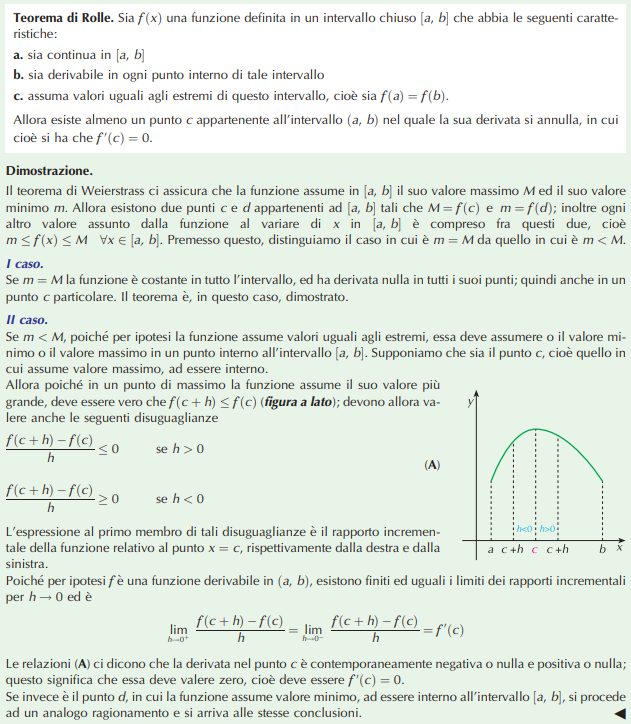
\includegraphics[width=\linewidth]{../dim/Rolle.PNG}
\end{figure}
\newpage
\subsection*{Teorema di Lagrange o del valor medio}
Enunciato:\newline
Sia $f$ derivabile in $(a,b)$ e continua in $[a,b]$. Allora esiste $c \in (a,b)$ tale che 
\[
    \frac{f(b)-f(a)}{b-a}= f'(c)
\]
Dimostrazione:\newline
\begin{figure}[h!]
    \includegraphics[width=\linewidth]{../dim/lagrange.PNG}
\end{figure}
\newpage
\subsection*{Test di monotonia su un intervallo}
Enunciato:\newline
Sia $f:(a,b) \rightarrow \mathbb{R}$, derivabile. Allora
\[
    f \;\; crescente \Leftrightarrow f'(x)\geq 0
\]
\[
    f \;\; decrescente \Leftrightarrow f'(x) \leq 0
\]
Dimostrazione:\newline
\begin{figure}[h!]
    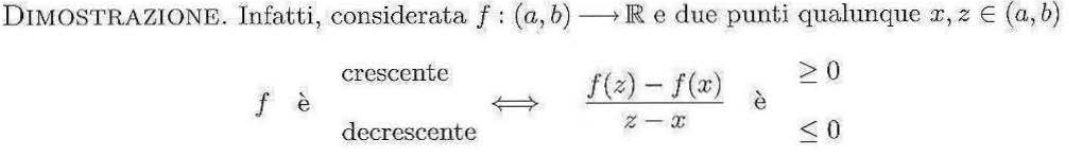
\includegraphics[width=\linewidth]{../dim/monotonia1.PNG}
\end{figure}
\newline\begin{figure}[h!]
    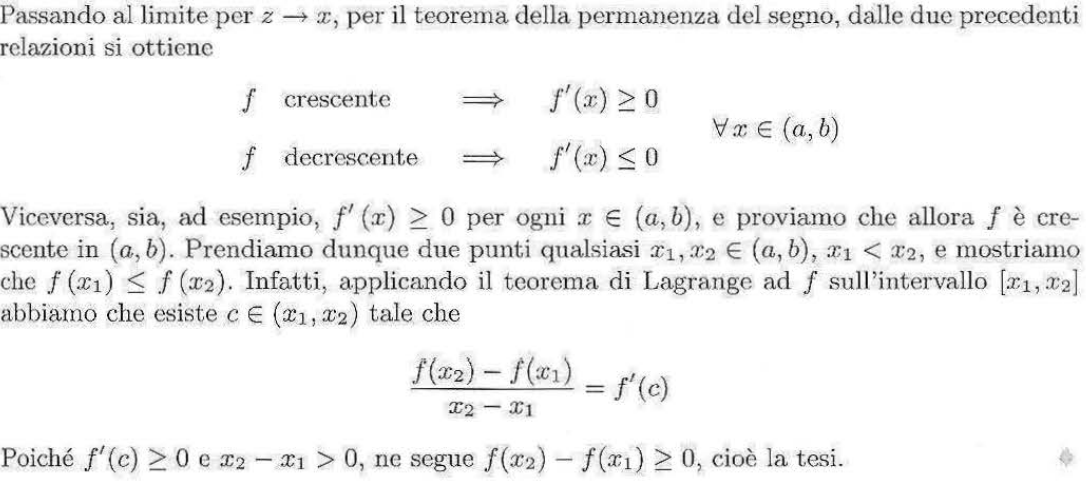
\includegraphics[width=\linewidth]{../dim/monotonia2.PNG}
\end{figure}
\newpage
\subsection*{Teorema di Cauchy}
\begin{figure}[h!]
    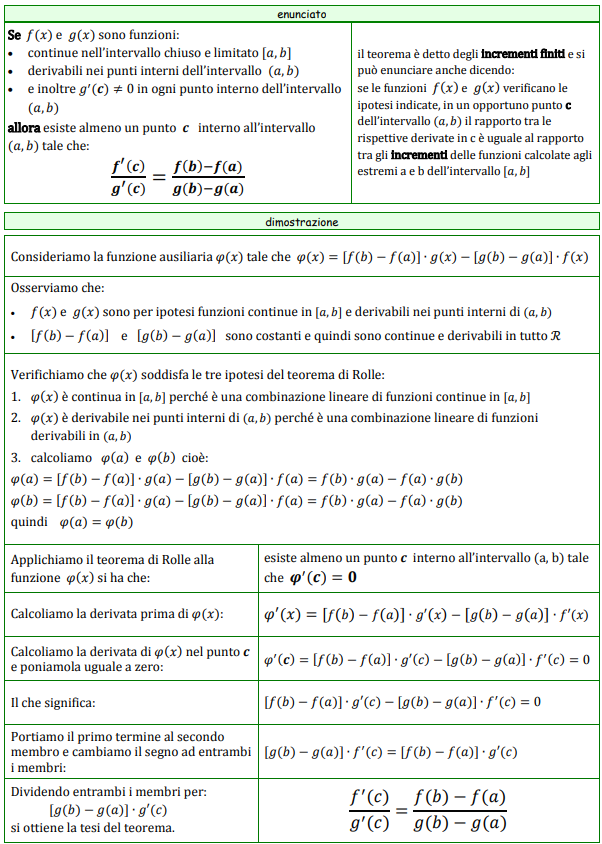
\includegraphics[width=\linewidth]{../dim/cauchy.PNG}
\end{figure}
\newpage
\subsection*{Teorema di l'Hospital}
Enunciato:\newline
Siano $f, g$ funzioni derivabili in un intervallo $(a,b)$, con $g,g' \neq 0$ in $(a,b)$. Se
\[
    \lim_{x\rightarrow a^+}f(x) = \lim_{x\rightarrow a^-}g(x) = 0 \;\;oppure \;\;\pm \infty
\]
e
\[
    \lim_{x\rightarrow a^+} \frac{f'(x)}{g'(x)}= L
\]
Allora 
\[
    \lim_{x\rightarrow a^+} \frac{f(x)}{g(x)} = L
\]
Il teorema è applicabile anche se $a \rightarrow -\infty$ oppure se si considera il limite per $x \rightarrow b^-$ (anzichè per $x \rightarrow  a^+$), con $b\leq + \infty$.
Dimostrazione:\newline
Sia $x_n$ una successione tendente ad $a^+$, prolunghiamo per continuità $f$ e $g$ in $a$ ponendo $f(a) = g(a) = 0$. Allora
\[
    \frac{f(x-n)}{g(x_n)} = \frac{f(x_n) -f(a)}{g(x_n)-g(a)}
\]
Se applichiamo a $f,g$ separatemente il teorema di lagrange sull'intervallo $[a, x_n]$, otteniamo che l'ultimo quoziente scritto è uguale a:
\[
    \frac{f'(t_n)(x_n -a)}{g'(t_n^*)(x_n-a)} = \frac{f'(t_n)}{g'(t_n^*)}
\]
dove $t_n, t_n^*$ sono fue punti opportuni che cadono nell'intervallo $(a,x_n)$. Poichè quando $x_n \rightarrow 0$ anche $t_n$ e $t_n^*\rightarrow 0$, sembra "ragionevole" che il limite del quoziente $\frac{f'}{g'}$ sia uguale al limite del quoziente $\frac{f}{g}$. Tuttavia questo non si può affermare rigorosamente, perchè le successioni $t_n, t_n^*$ sono a priori diverse tra loro. Per aggirare il problema occorre modificare leggermente l'argomentazione seguita. Riprendiamo dunque la dimostrazione della $\frac{f(x-n)}{g(x_n)} = \frac{f(x_n) -f(a)}{g(x_n)-g(a)}$, e definiamo
\[
    h(x) = f(x_n) g(x) - g(x_n) f(x)
\]
Notiamo che $h(a) = h(x_n) = 0$. La funzione $h$ soddisfa le ipotesi del teorema di lagrange sull'intervallo $[a,x_n]$, dunque esiste $t_n \in(a,x_n)$ tale che 
\[
    h'(t_n) = \frac{f(x_n) - h(a)}{x_n-a} = 0
\]
ovvero, calcolando
\[
    h'(x) = f(x_n)g'(x) -g(x_n) f'(x), \;\;\;\;\;\; f(x_n)g'(t_n)-g(x_n)f'(t_n) = 0
\]
Dunque per ogni $x_n$ esiste un punto $t_n \in (a,x_n)$ tale che 
\[
    \frac{f(x_n)}{g(x_n)} = \frac{f'(t_n)}{g'(t_n)}
\]
Per $n \rightarrow  \infty$, $t_n \rightarrow a^+$, perciò $\frac{f'(t_n)}{g'(t_n)} \rightarrow L$, e di conseguenza anche $\frac{f(x_n)}{g(x_n)} \rightarrow L$, che è quanto volevamo dimostrare.
\newpage
\subsection*{Formula di Taylor con resto secondo Peano}
\begin{figure}[h!]
    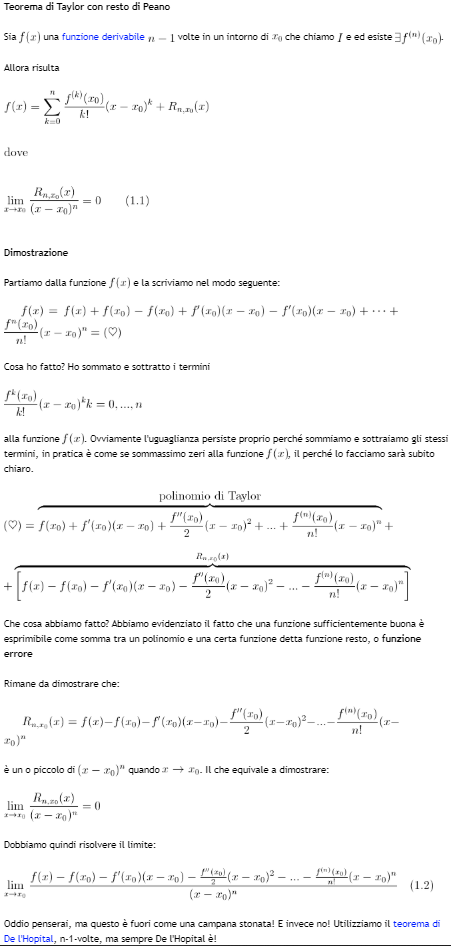
\includegraphics[width=300px]{../dim/taylorpeano1.PNG}
\end{figure}
\newpage
\begin{figure}[h!]
    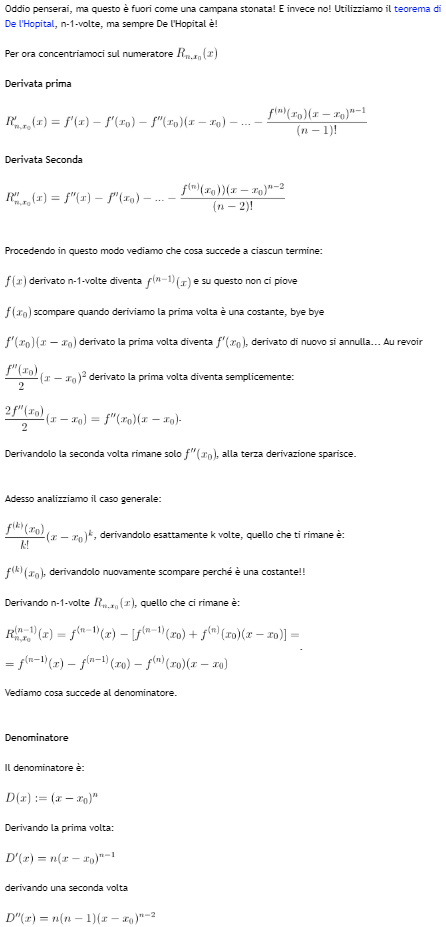
\includegraphics[width=300px]{../dim/taylorpeano2.PNG}
\end{figure}
\newpage
\begin{figure}[h!]
    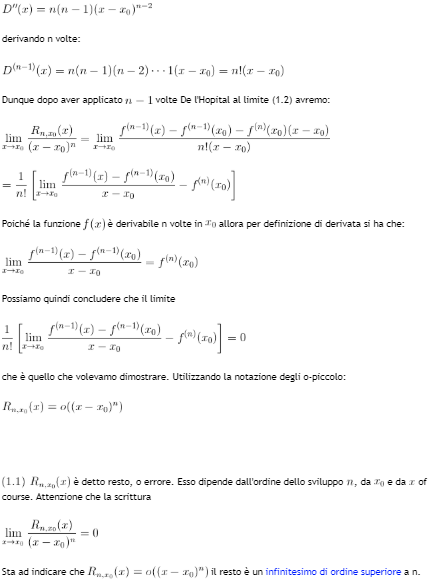
\includegraphics[width=300px]{../dim/taylorpeano3.PNG}
\end{figure}
\newpage
\subsection*{Formula di Taylor con resto secondo Lagrange}
Enunciato:
\begin{figure}[h!]
    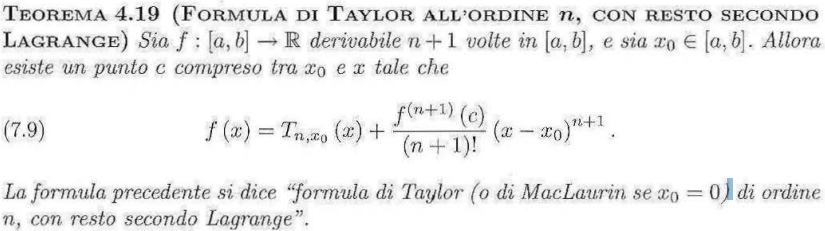
\includegraphics[width=\linewidth]{../dim/taylorlagrange1.PNG}
\end{figure}
\newline
Dimostrazione:\begin{figure}[h!]
    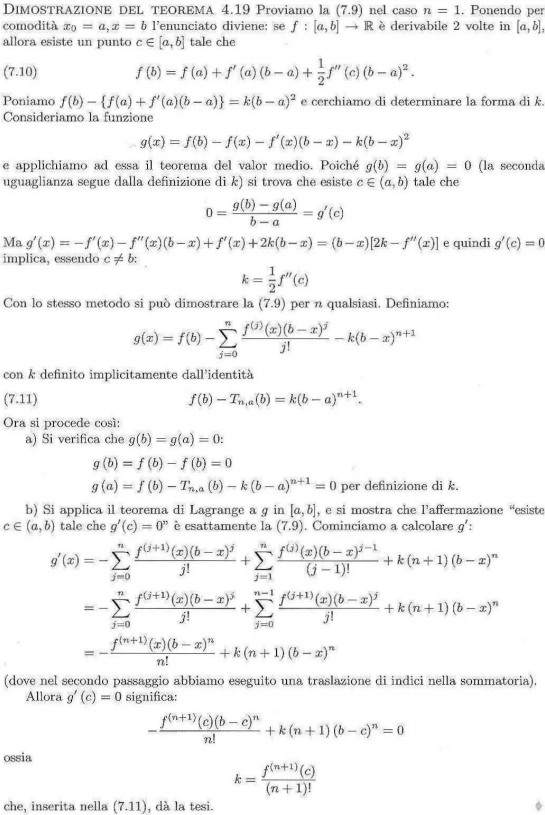
\includegraphics[width=300px]{../dim/taylorlagrange2.PNG}
\end{figure}
\newline
\newpage
\subsection*{Primo teorema fondamentale del calcolo integrale}
Enunciato:\begin{figure}[h!]
    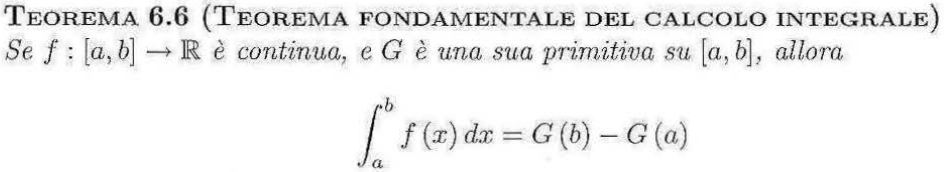
\includegraphics[width=\linewidth]{../dim/integrale1.PNG}
\end{figure}
\newline
Dimostrazione:\begin{figure}[h!]
    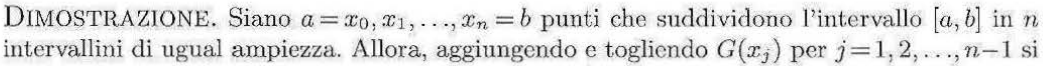
\includegraphics[width=\linewidth]{../dim/integrale2.PNG}
\end{figure}
\newline\begin{figure}[h!]
    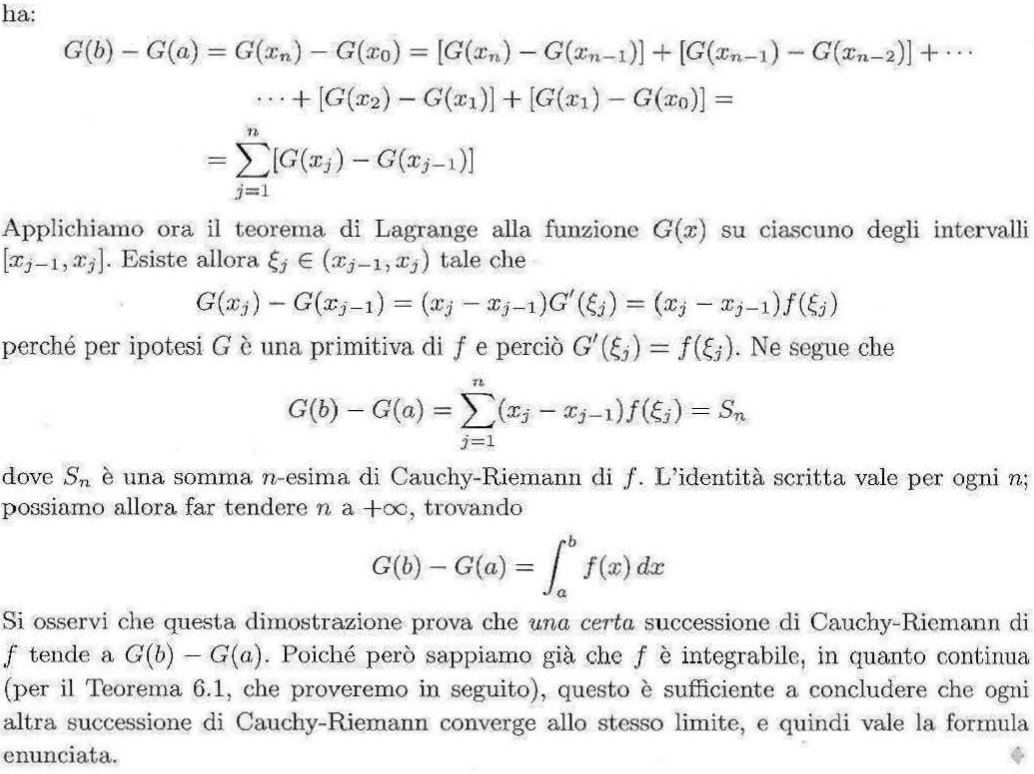
\includegraphics[width=\linewidth]{../dim/integrale3.PNG}
\end{figure}
\newpage
\subsection*{Condizione necessaria per la convergenza delle serie}\begin{figure}[h!]
    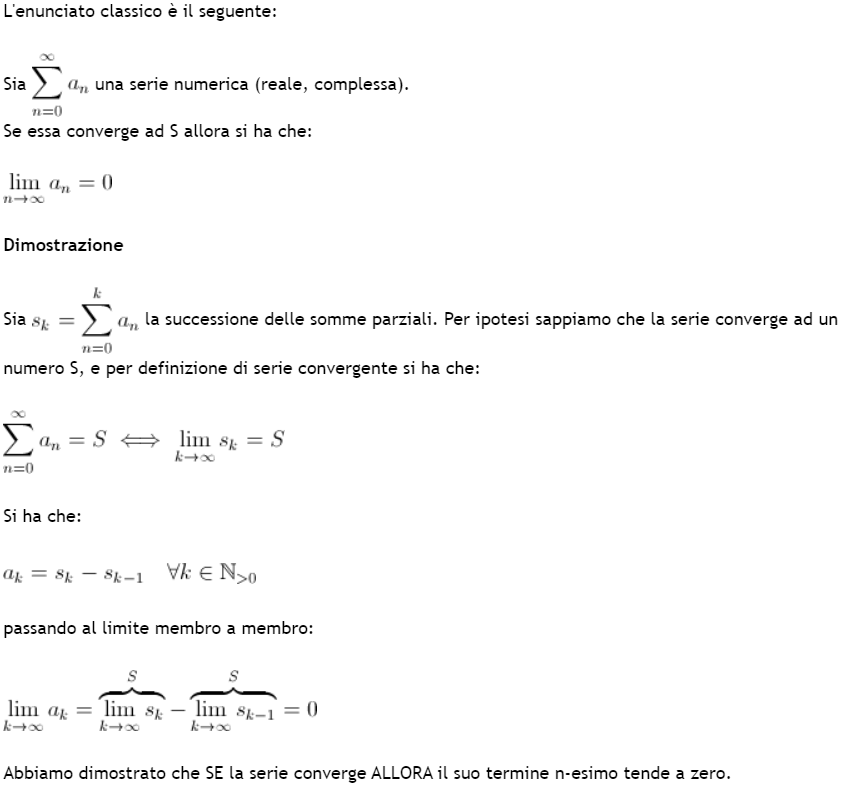
\includegraphics[width=\linewidth]{../dim/convserie.PNG}
\end{figure}
\newpage
\subsection*{Criterio del rapporto per la convergenza delle serie a termini positivi}
Enunciato:\begin{figure}[h!]
    
\includegraphics[width=\linewidth]{../dim/rapporto1.PNG}
\end{figure}
\newline
Dimostrazione:\begin{figure}[h!]
    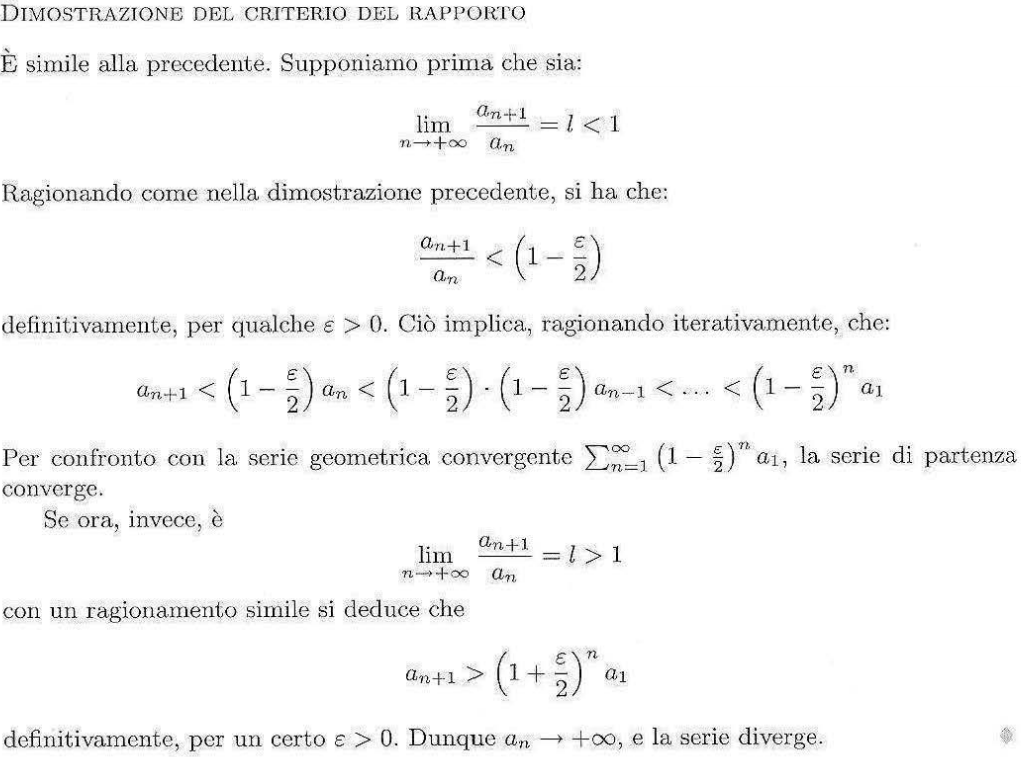
\includegraphics[width=\linewidth]{../dim/rapporto2.PNG}
\end{figure}
\newpage
\subsection*{Criterio del confronto per la convergenza di una serie a termini positivi}
Enunciato:\begin{figure}[h!]
    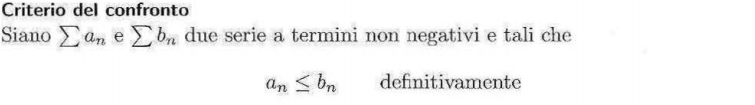
\includegraphics[width=\linewidth]{../dim/confronto1.PNG}
\end{figure}
\newline\begin{figure}[h!]
    
\includegraphics[width=\linewidth]{../dim/confronto2.PNG}
\end{figure}
\newline
Dimostrazione:\begin{figure}[h!]
    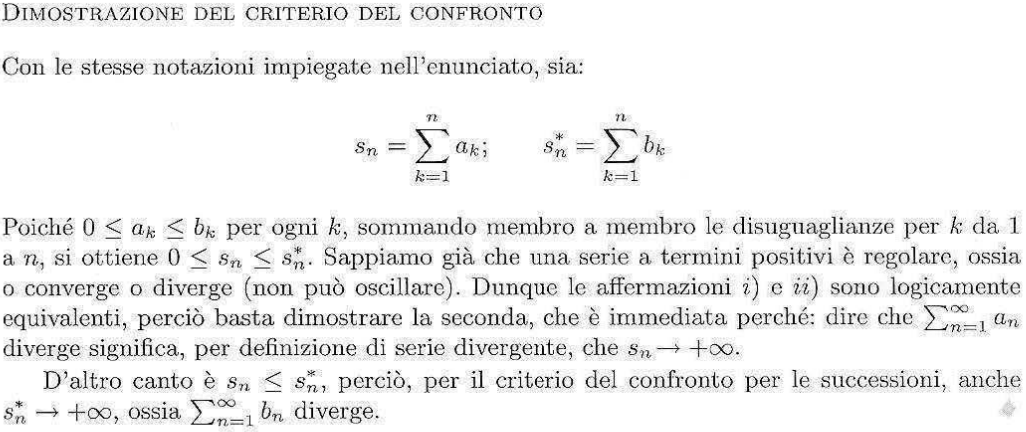
\includegraphics[width=\linewidth]{../dim/confronto3.PNG}
\end{figure}
\newpage
\subsection*{Criterio della radice per la convergenza della serie a termini positivi}
Enunciato:\begin{figure}[h!]
    
\includegraphics[width=\linewidth]{../dim/radice1.PNG}
\end{figure}
\newline
Dimostrazione:\begin{figure}[h!]
    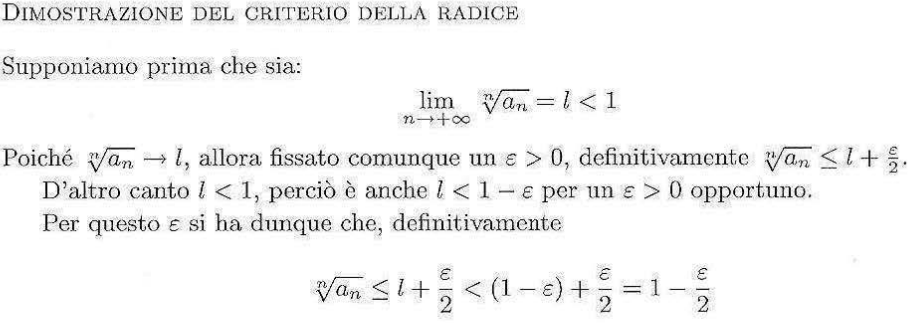
\includegraphics[width=\linewidth]{../dim/radice2.PNG}
\end{figure}
\newline
\begin{figure}[h!]
    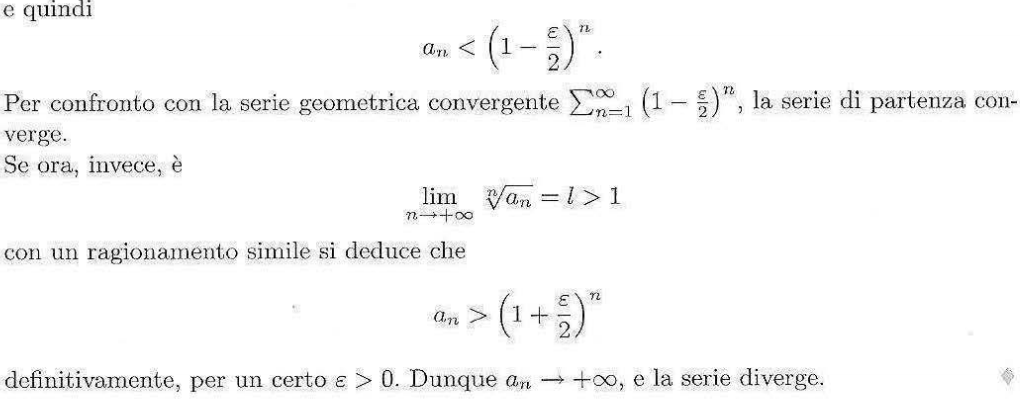
\includegraphics[width=\linewidth]{../dim/radice3.PNG}
\end{figure}
\newpage
\subsection*{Giustificazione della formula di Eulero con l’esponenziale complesso}
Enunciato:
\begin{figure}[h!]
    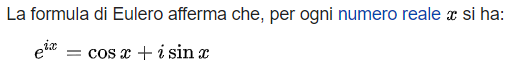
\includegraphics[width=\linewidth]{../dim/eulero1.PNG}
\end{figure}
\newline
Dimostrazione:\begin{figure}[h!]
    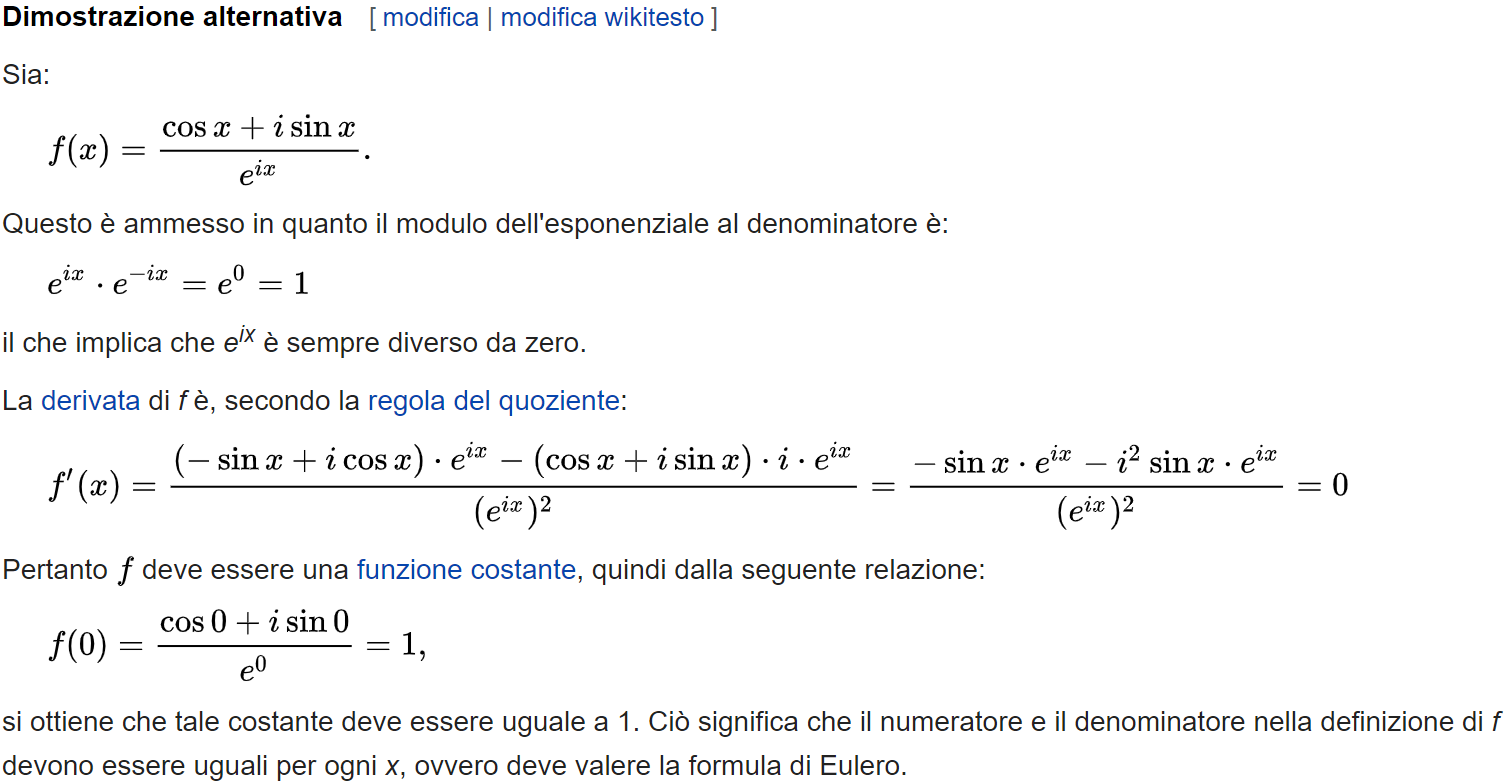
\includegraphics[width=\linewidth]{../dim/eulero2.PNG}
\end{figure}
\newline
\end{document}